\section{Implementierung}
\label{sec:implementation}
\subsection{List-based set with coarse-grained locks}

Bei dieser Implementierung wir vor jedem Methodenaufruf die gesammte Liste gesperrt. Dadurch kann aber die Parallelisierung nicht wirklich ausgenutzt werden, da zu einem Zeitpunkt maximal ein Prozess auf die Liste zugreifen kann. Diese Implementierung ist daher sehr ähnlich zu einer sequentiellen Implementierung.

\begin{figure}[H]
	\centering
    \begin{tikzpicture}
        \draw (-0.5,1) -- (10.5,1) node [midway, above, sloped] {\faLock};
		\node[draw,circle,minimum size=1cm,inner sep=0pt] at (0,0) {$- \infty$};
		\draw[->] (0.5,0) -- (1.5,0);
		\node[draw,circle,minimum size=1cm,inner sep=0pt] at (2,0) {$3$};
		\draw[->] (2.5,0) -- (3.5,0);
		\node[draw,circle,minimum size=1cm,inner sep=0pt] at (4,0) {$5$};
		\draw[->] (4.5,0) -- (5.5,0);
		\node[draw,circle,minimum size=1cm,inner sep=0pt] at (6,0) {$8$};
		\draw[->] (6.5,0) -- (7.5,0);
		\node[draw,circle,minimum size=1cm,inner sep=0pt] at (8,0) {$10$};
		\draw[->] (8.5,0) -- (9.5,0);
		\node[draw,circle,minimum size=1cm,inner sep=0pt] at (10,0) {$\infty$};
	\end{tikzpicture}
	\caption{coarse-grained locks}
	\label{tik:coarse-grained}
\end{figure}

\begin{table}[H]
    \begin{tabularx}{\textwidth}{lX}
        \textbf{Linearisation Point} & Die Sperrung\\
        \\
        \textit{add} & Nachdem die Liste gegsperrt wurde wird sie durchlaufen bis zu dem Punkt an dem der Key der betrachteten Node größer ist als der Einzufügende. Dort wird die Neue Node eingefügt. \\
        \textit{contains} & Die Liste wird gesperrt und dann durchlaufen. Wenn dabei der gesuchten Wert gefunden wird, wird \textit{true} sont \textit{false} zurückgegeben.\\
        \textit{remove} & Nachdem die gesamte Liste gesperrt wurde wird das Element in der Liste gesucht und entfernt.\\
    \end{tabularx}
\end{table}

\subsection{List-based set with fine-grained locks}

Im Unterschied zu den coarse-grained locks wird bei dieser Implementierung immer nur die derzeitige Node gesprerrt. 
Beim Iterieren der Liste wird während dem Übergang zur nächsten Node die derzeitige und die darauffolgende Node gesperrt. 
Eine Node kann zu einem Zeitpunkt nur von einem Prozess gesperrt sein. Der Vorteil gegenüber den coarse-grained locks besteht darin, 
dass nun wirkliche Parallelisierung möglich ist und verschiedene Threads an unterschiedlichen Punkten an der Liste arbeiten können. 
Es hat jedoch den Nachteil, dass die Iterationsgeschwiendigkeit im Worst Case durch den langsamsten Thread definiert wird, da ein 
Thread in der Liste nicht ``Überholt'' werden kann.

\begin{figure}[H]
	\centering
    \begin{tikzpicture}
        \draw (3.5,1) -- (4.5,1) node [midway, above, sloped] {\faLock};
        \draw (5.5,1) -- (6.5,1) node [midway, above, sloped] {\faLock};
		\node[draw,circle,minimum size=1cm,inner sep=0pt] at (0,0) {$- \infty$};
		\draw[->] (0.5,0) -- (1.5,0);
		\node[draw,circle,minimum size=1cm,inner sep=0pt] at (2,0) {$3$};
		\draw[->] (2.5,0) -- (3.5,0);
		\node[draw,circle,minimum size=1cm,inner sep=0pt] at (4,0) {$5$};
		\draw[->] (4.5,0) -- (5.5,0);
		\node[draw,circle,minimum size=1cm,inner sep=0pt] at (6,0) {$8$};
		\draw[->] (6.5,0) -- (7.5,0);
		\node[draw,circle,minimum size=1cm,inner sep=0pt] at (8,0) {$10$};
		\draw[->] (8.5,0) -- (9.5,0);
		\node[draw,circle,minimum size=1cm,inner sep=0pt] at (10,0) {$\infty$};
	\end{tikzpicture}
	\caption{fine-grained locks}
	\label{tik:fine-grained}
\end{figure}

\begin{figure}[H]
	\centering
    \begin{tikzpicture}
        \draw (3.5,1) -- (4.5,1) node [midway, above, sloped] {\faLock};
        \draw (5.5,-1) -- (6.5,-1) node [midway, above, sloped] {\faLock};
		\node[draw,circle,minimum size=1cm,inner sep=0pt] at (0,0) {$- \infty$};
		\draw[->] (0.5,0) -- (1.5,0);
		\node[draw,circle,minimum size=1cm,inner sep=0pt] at (2,0) {$3$};
		\draw[->] (2.5,0) -- (3.5,0);
		\node[draw,circle,minimum size=1cm,inner sep=0pt] at (4,0) {$5$};
        \draw[->] (4.5,0) -- (7.5,0);
        \draw[line width=0.5mm, red] (5.5,-1.5) -- (6.5,-2.5);
        \node[draw,circle,minimum size=1cm,inner sep=0pt] (A) at (6,-2) {$8$};
        \node[draw,circle,minimum size=1cm,inner sep=0pt] (B) at (8,0) {$10$};
        \draw[->] (A) -- (B);
		\draw[->] (8.5,0) -- (9.5,0);
		\node[draw,circle,minimum size=1cm,inner sep=0pt] at (10,0) {$\infty$};
	\end{tikzpicture}
	\caption{fine-grained locks remove}
	\label{tik:fine-grained-remove}
\end{figure}

\begin{table}[H]
    \begin{tabularx}{\textwidth}{lX}
        \textbf{Linearisation Point} & Wenn der Key in der Liste ist dann der Punkt an dem die zu suchende Node gesperrt wurde. Sonst wenn die nächst höhere Node gesperrt wurde.\\
        \\
        \textit{add} & Die Liste wird iteriert und an dem Punkt an dem die Node eingefügt werden soll wird sowohl der Vorgänger als auch der Nachfolger gesperrt. Dadurch kann die neue Node sicher eingefügt werden.\\
        \textit{contains} & Die Liste wird analog zur coarse-grained locks iteriert dabei aber immer die derzeitige Node bzw. beim Übergang Vorgänger und Nachfolger gesperrt. Wenn die entwprechende Node gefunden wurde wird \textit{true} sonst \textit{false} zurückgegeben. \\
        \textit{remove} & Die Liste wird wie bei contains iteriert und wenn die zu entfernende Node gefunden wurde wird der Zeiger der Vorgänger Node auf den darauffolgenden verwiesen und somit die zu entfernende Node übersprungen. Siehe in Abbildung \ref{tik:fine-grained-remove}\\
    \end{tabularx}
\end{table}

Diese Implementierung setzt Memory Management vorraus. Dies ist in Kapitel \ref{sec:mem} genauer beschrieben.

\subsection{List-based set with optimistic synchronization}

In dieser Implementierung wird beim Suchen eines ELementes zuerst keine Node gesperrt sonder einfach nur eine Iteration durchgeführt. Sobald das gesuchte gefunden wurde wird dieses gesperrt und sichergestellt, dass diese Node immernoch erreichbar ist. Falls dies nicht der Fall sein sollte wird startet der Algorithmus von vorne.

\begin{table}[H]
    \begin{tabularx}{\textwidth}{lX}
        \textbf{Linearisation Point} & ???\\
        \\
        \textit{add} & \\
        \textit{contains} & \\
        \textit{remove} & \\
    \end{tabularx}
\end{table}

\subsection{List-based set with lazy synchronization}

Lazy Synchronization verwendet eine Markierung auf den Nodes die bekannt gibt ob diese Node noch aktiv ist oder nicht. Bei einem Lösch Vorgang wird bei der zu löschenden Node diese Markierung gesetzt. Dadurch wird diese Node bei anderen Methoden, wie zum Beispiel Contains oder Add, ignoriert. 

In späterer folge wird durch das Memory management, ähnlich wie bei optimistic synchronization, die Node gelöscht sobald sichergestellt werden kann, dass kein Process mehr auf die Node zugreift.

\begin{table}[H]
    \begin{tabularx}{\textwidth}{lX}
        \textbf{Linearisation Point} & ???\\
        \\
        \textit{add} & \\
        \textit{contains} & \\
        \textit{remove} & \\
    \end{tabularx}
\end{table}

\subsection{Lock-free list-based set}

\begin{table}[H]
    \begin{tabularx}{\textwidth}{lX}
        \textbf{Linearisation Point} & ???\\
        \\
        \textit{add} & \\
        \textit{contains} & \\
        \textit{remove} & \\
    \end{tabularx}
\end{table}